\subsection{Dataset Collection}

\noindent Our dataset acquisition process involved the following steps:


\subsubsection{Public Datasets}
A significant part of our extensive dataset was thoughtfully put together from openly accessible collections of deepfake and authentic images. We carefully chose these datasets to make our deepfake detection model more diverse and applicable. This approach helps us ensure a strong and thorough training and testing process by making the most of these available resources.

% Here's the breakdown of our dataset:
% % \begin{itemize}
% %     \item \textbf{Trained:} 70,000 samples
% %     \item \textbf{Tested:} 5,000 samples
% %     \item \textbf{Validation:} 15,000 samples
% % \end{itemize}
% Our dataset contains data from well-known public sources, and each of these sources has a specific role in making our deepfake detection system better :

\begin{enumerate}
\item \textbf{CelebA:} CelebA is a large-scale face attributes dataset with annotations for 40 attributes, commonly used for facial recognition and generative tasks.

\item \textbf{FFHQ (Flickr-Faces-HQ):} FFHQ is a high-resolution face dataset containing 70,000 images from diverse identities, frequently utilized for training high-quality face generation models.

\item \textbf{StarGAN:} StarGAN is a dataset for image-to-image translation tasks, facilitating research in image translation, domain adaptation, and style transfer.

\item \textbf{AttGAN:} AttGAN is a dataset designed for facial attribute manipulation, providing images with annotations for training models in attribute-based image editing.

\item \textbf{StyleGAN:} StyleGAN is a dataset used with the StyleGAN model, capable of generating diverse and high-quality images, popular for art generation and creative applications.

\item \textbf{StyleGAN2:} StyleGAN2 is an enhanced version of StyleGAN, producing higher quality and more realistic images, widely used for generative image synthesis.

\end{enumerate}


\subsubsection{Video Conversion}
To include videos in our dataset, we first converted them into individual frames (images) to facilitate compatibility with the vision transformer architecture. This step involved extracting frames at a consistent frame rate from each video, resulting in a sequence of images for each video.
\begin{figure}[htbp]
    \centering
    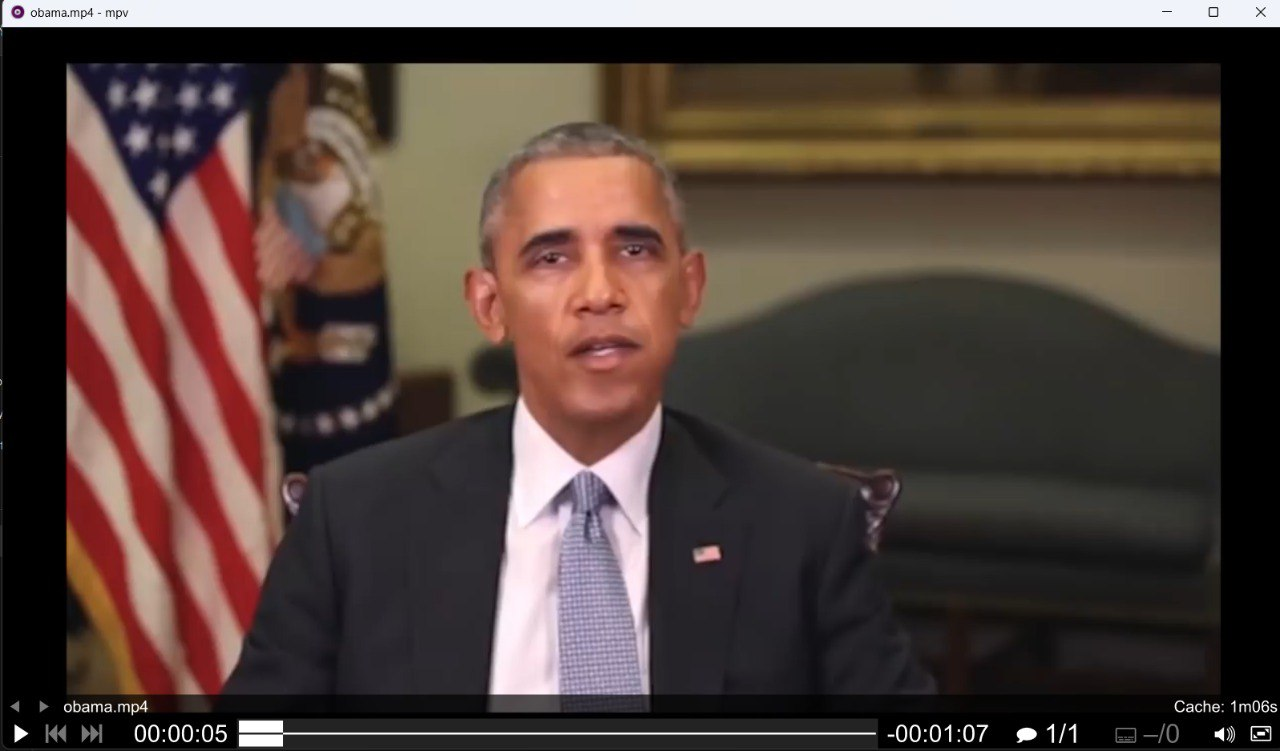
\includegraphics[width= 5in ]{img/framesExtracted.jpg}
    \caption{\textit{Video Sample}}
\end{figure}
\begin{figure}[ht]
    \centering
    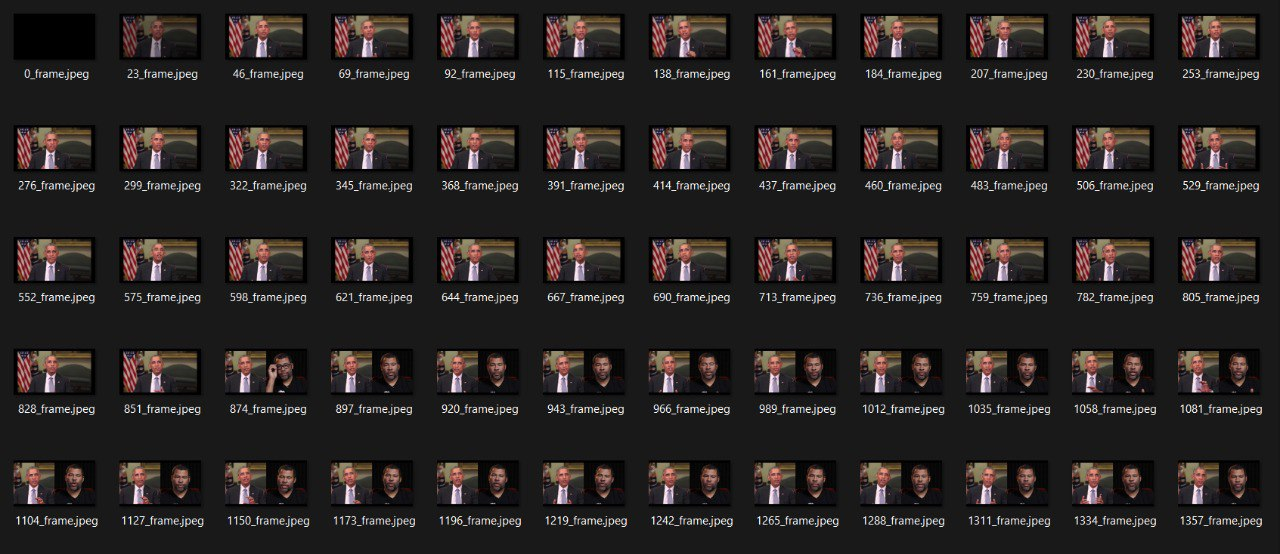
\includegraphics[width= 5in ]{img/frames.jpg}
    \caption{\textit{Frames Extracted from video}}
\end{figure}

\subsubsection{Frame Selection}
To avoid redundancy and maintain dataset balance, we carefully selected frames from videos to represent various stages of manipulation, expressions, poses, and lighting conditions.

\begin{figure}[htbp]
    \centering
    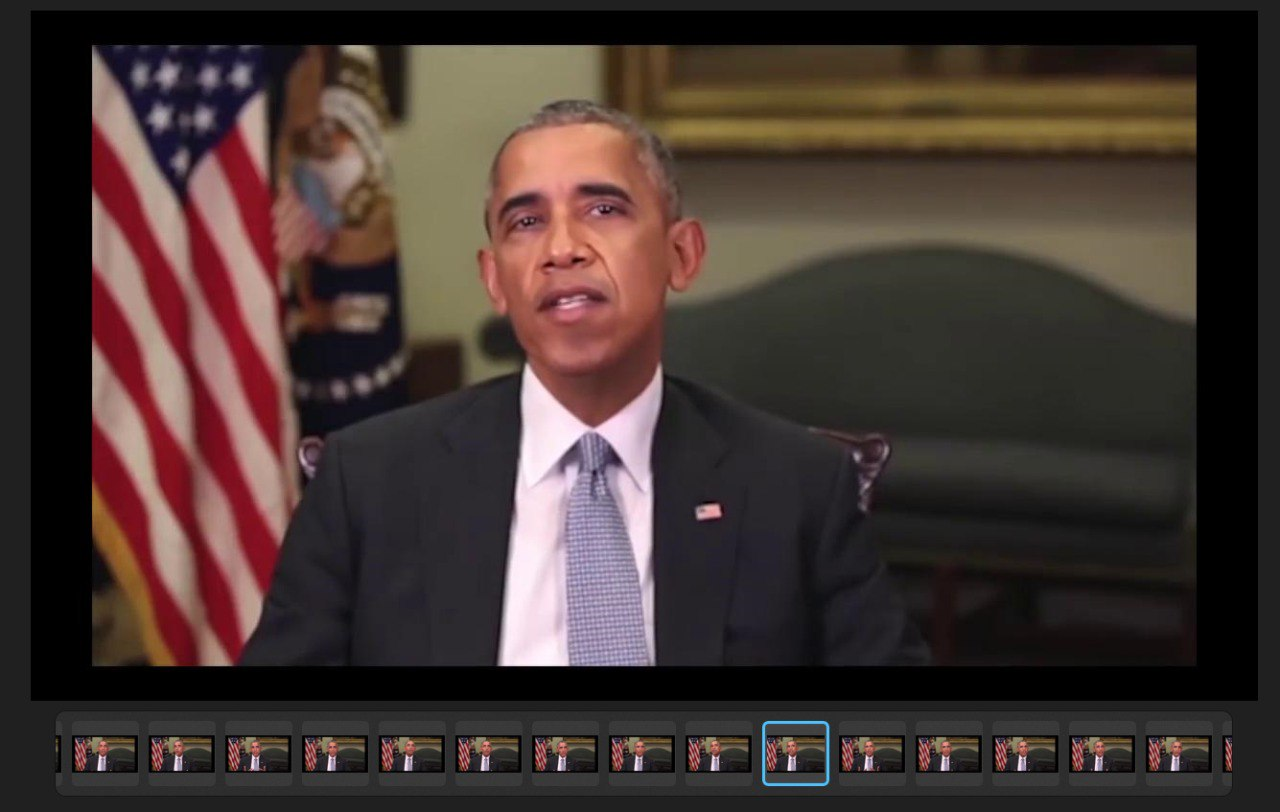
\includegraphics[width= 5in ]{img/frameSelected.jpg}
    \caption{Seleting required frames}
\end{figure}


\subsubsection{Annotation and Labeling}
Each image was labeled as either "real" or "deepfake." Annotations were done manually to ensure accurate labeling for training and evaluation.

\newpage